\documentclass[a4paper,12pt]{article}
\newcommand{\cName}{Jenish Pant} % Name of the student
\newcommand{\cRollNo}{THA078BEI018} % Roll no. of the student
\newcommand{\cSubj}{Computer Network} % Subject
\newcommand{\cLabNumber}{4}
\newcommand{\cSubmissionDate}{\today} % Submission date
\newcommand{\cTitle}{SETTING PASSWORD IN ROUTER AND SETTING UP DHCP SERVER IN CISCO PACKET TRACER}
\title{Lab4: Setting Password in Router and Setting up DHCP Server in Cisco Packet Tracer}
\author{\cName}


\usepackage{graphicx} % For including images
\usepackage{amsmath} % For better math support
\usepackage[a4paper]{geometry}

\geometry{
  textwidth=\dimexpr\paperwidth-29mm,
  textheight=\dimexpr\paperheight-32mm,
  noheadfoot,
  nomarginpar
}

\setlength{\topskip}{0mm}
\setlength{\parindent}{0mm}

\title{Lab \cLabNumber: \cTitle}
\date{}
\author{}
\begin{document}

\maketitle
\vspace{-2cm}
\section*{INTRODUCTION}
In this lab, we will learn how to set a password on a router and how to set up a DHCP server in Cisco Packet Tracer.

\section*{OBJECTIVES}
\begin{itemize}
    \item To understand the importance of setting a password on a router.
    \item To learn how to set a password on a router in Cisco Packet Tracer.
    \item To understand the role of a DHCP server in a network.
    \item To learn how to set up a DHCP server in Cisco Packet Tracer.
\end{itemize}

\section*{THEORY}

\subsubsection*{Setting up a Normal Password}
A normal password, also known as the console password, is used to secure access to the router's console port. This password is required when you want to log into the router via the console port. The console port is a physical interface on the router that allows for direct device management.

\begin{verbatim}
Router> enable
Router# configure terminal
Router(config)# enable password PASSWORD
Router(config)# exit
\end{verbatim}



\subsubsection*{Setting up a Telnet (VTY) Password}
A Telnet password, also known as a VTY password, is used to secure remote access to the router. This password is required when you want to log into the router remotely via Telnet. Telnet is a protocol that allows for remote device management.



\begin{verbatim}
Router> enable
Router# configure terminal
Router(config)# line vty 0 4
Router(config-line)# password PASSWORD
Router(config-line)# login
Router(config-line)# exit
\end{verbatim}


\subsubsection*{Setting up a Secret Password}
A secret password is used to secure privileged access to the router. This password is required when you want to enter the privileged EXEC mode on the router. The privileged EXEC mode allows for full control over the router, including the ability to view and modify the router's configuration.

\begin{verbatim}
Router> enable
Router# configure terminal
Router(config)# enable secret PASSWORD
Router(config)# exit
\end{verbatim}




\subsection*{Setting up a DHCP Server}
A DHCP (Dynamic Host Configuration Protocol) server automatically assigns IP addresses to devices on a network. This eliminates the need for network administrators to manually assign IP addresses to every device on the network. In Cisco Packet Tracer, we can set up a DHCP server using the following commands:

\begin{verbatim}
Router> enable
Router# configure terminal
Router(config)# ip dhcp pool POOLNAME
Router(dhcp-config)# network NETWORK_ADDRESS SUBNET_MASK
Router(dhcp-config)# default-router DEFAULT_ROUTER_ADDRESS
Router(dhcp-config)# exit
Router(config)# exit
\end{verbatim}




\section*{PROCEDURE}
\begin{enumerate}
    \item Create a new network topology in Cisco Packet Tracer.
    \item Configure the router with a password.
    \item Set up a DHCP server on the router.
    \item Test the network connectivity.
\end{enumerate}

\section*{RESULTS}
\begin{itemize}
    \item Successfully created a new network topology in Cisco Packet Tracer.
    \item Configured the router with a password.
    \item Set up a DHCP server on the router.
    \item Verified network connectivity.

          \begin{figure}[!ht]
              \centering
              \begin{minipage}{0.45\textwidth}
                  \centering
                  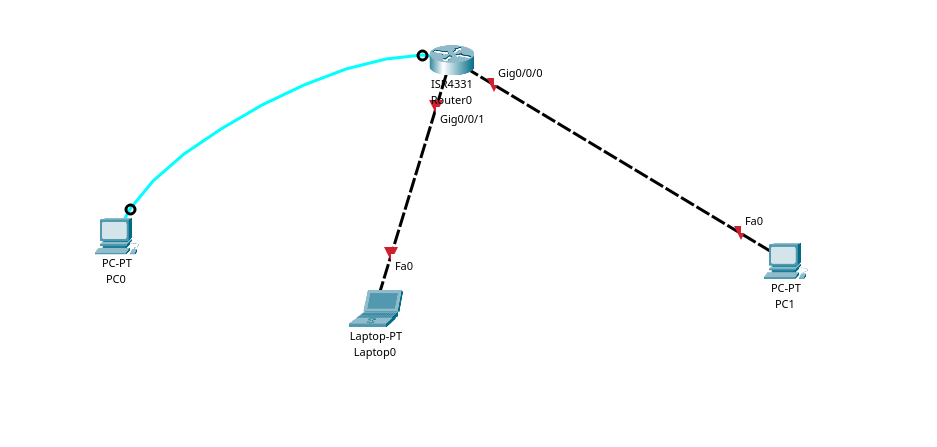
\includegraphics[width=\textwidth]{img/topology.png}
                  \caption{Network Topology}
                  \label{fig:network_topology}
              \end{minipage}\hfill
              \begin{minipage}{0.45\textwidth}
                  \centering
                  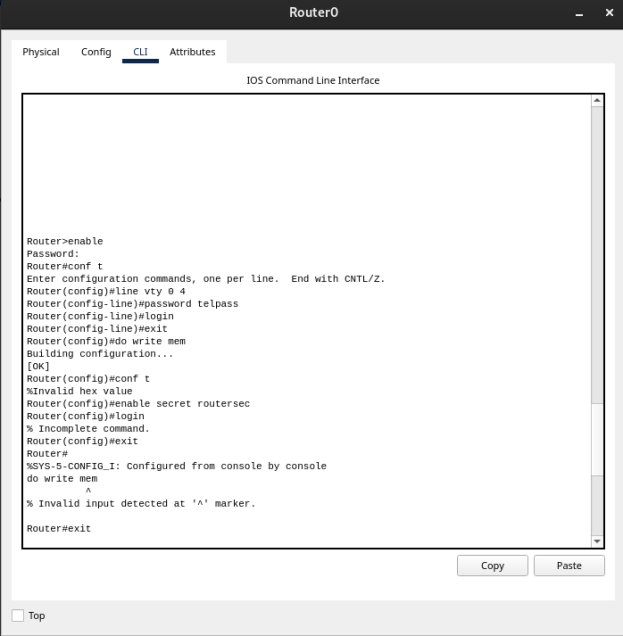
\includegraphics[width=\textwidth]{img/enable_password.png}
                  \caption{Configured Router Password}
                  \label{fig:router_password}
              \end{minipage}
          \end{figure}

          \begin{figure}[!ht]
              \centering
              \begin{minipage}{0.45\textwidth}
                  \centering
                  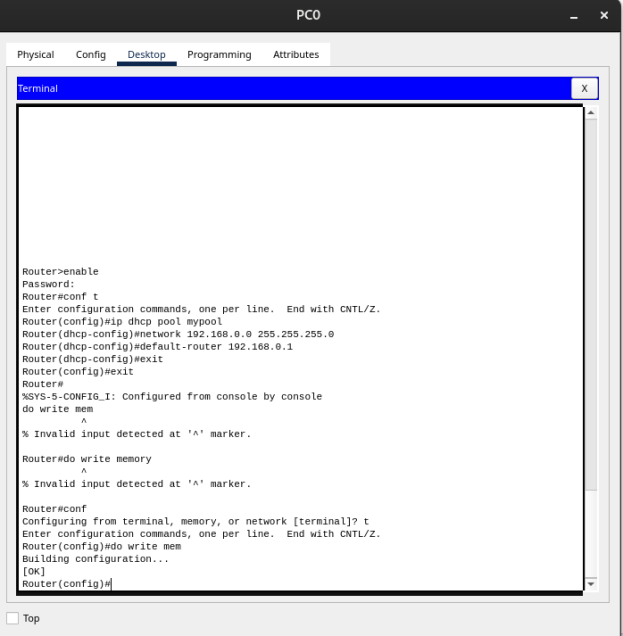
\includegraphics[width=\textwidth]{img/enable_secret.png}
                  \caption{Configured Router Secret}
                  \label{fig:router_secret}
              \end{minipage}\hfill
              \begin{minipage}{0.45\textwidth}
                  \centering
                  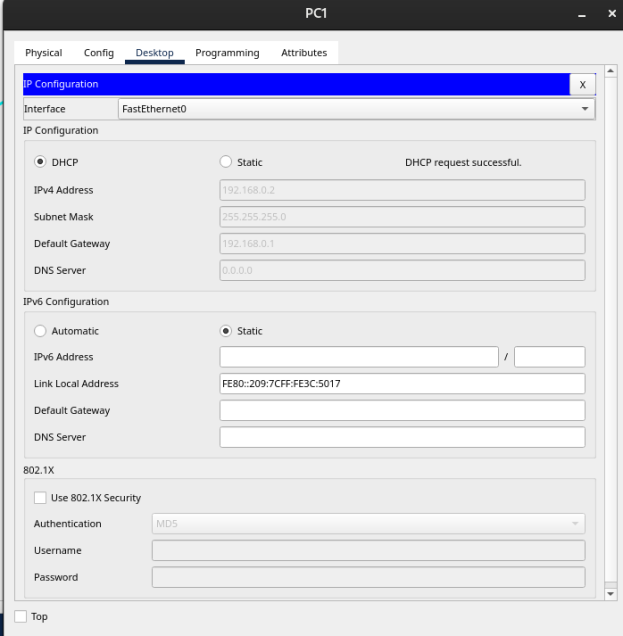
\includegraphics[width=\textwidth]{img/dhcp.png}
                  \caption{Setting up a DHCP Server}
                  \label{fig:dhcp_server}
              \end{minipage}
          \end{figure}

		  \begin{figure}[!ht]
              \centering
              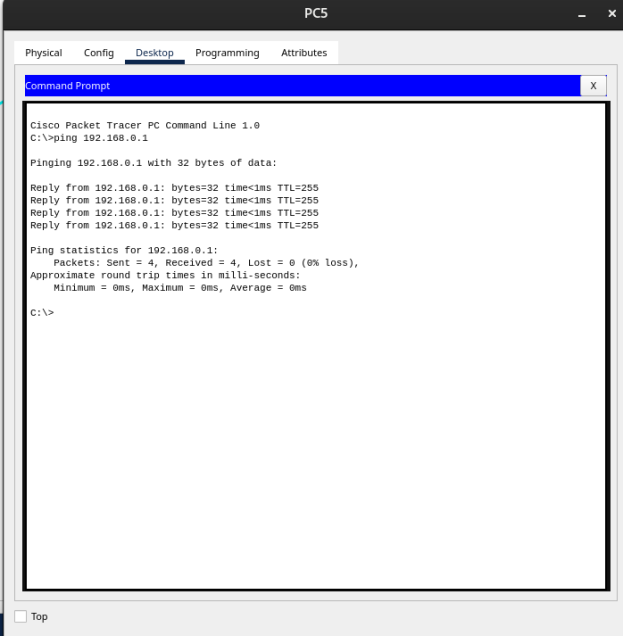
\includegraphics[width=0.5\textwidth]{img/connectivity.png}
              \caption{Verification of Network Connectivity}
              \label{fig:network_connectivity}
          \end{figure}

\end{itemize}

\section*{CONCLUSION}
In this lab, we have learned how to set up different types of passwords on a router and how to set up a DHCP server. These are fundamental skills for network administration. By setting up passwords, we can secure access to the router and prevent unauthorized users from modifying the router's configuration. By setting up a DHCP server, we can automate the assignment of IP addresses to devices on the network, which can greatly simplify network management. By practicing these skills in Cisco Packet Tracer, we can gain practical experience in network administration and prepare for real-world networking tasks.

\end{document}
